\documentclass[5p,twocolumn]{elsarticle}
\usepackage{amsmath}
\usepackage{hyperref} % added [draft] to avoid compilation issues that happen if a link is split and appears in two pages
%\modulolinenumbers[5]
\addtolength{\textheight}{8mm}
\addtolength{\textwidth}{4mm}
\addtolength{\voffset}{-10mm}
\addtolength{\hoffset}{-3mm}

\bibliographystyle{elsarticle-num-names}


% ACM template
%
%\documentclass[acmtog,anonymous,timestamp,review]{acmart}
%
%\usepackage{booktabs} % For formal tables
%




% My TK added packages and commands

	\newif\ifcolorrevise
	
	\colorrevisetrue

	% for for using hyperref and elsarticle-num-names together in order to get \citeauthor to work
	\makeatletter
	\providecommand{\doi}[1]{%
	  \begingroup
	    \let\bibinfo\@secondoftwo
	    \urlstyle{rm}%
	    \href{http://dx.doi.org/#1}{%
	      doi:\discretionary{}{}{}%
	      \nolinkurl{#1}%
	    }%
	  \endgroup
	}
	\makeatother

	% have multiline subfigure captions be centered
	\usepackage[labelformat=parens]{subcaption} % subfigures
	\captionsetup[subfigure]{justification=centering}
	\captionsetup{subrefformat=parens} % pure refernce subfigure with parentheses: fig.10a and (b)
	%\renewcommand\thesubfigure{(\alph{subfigure})} % refernce subfigure always with parentheses: fig.10(a) and (b)

	\captionsetup[figure]{labelfont={bf},name={Fig.},labelsep=period} % use `Fig.' for figure subscript instead of `Figure'
	
	\usepackage[export]{adjustbox} % [right] alignment for includegraphics
	
	\usepackage{rotating} % turn env for rotating text in figures

	\usepackage{wrapfig} % inline figures

	% tables
	\usepackage{multirow} % multicolumn, multirow
	\usepackage{colortbl} % \cellcolor{<color>}
	\newcolumntype{C}[1]{>{\centering\arraybackslash}m{#1}}   %% centered
	\newcolumntype{R}[1]{>{\raggedleft\arraybackslash}m{#1}}  %% right aligned

	\usepackage[capitalise]{cleveref} % automatically add `Fig.'  etc before a reference.

        \usepackage{ amssymb } % \therefore
	
	\newcommand{\degree}{^\circ}
	
	\usepackage[binary-units]{siunitx} % mm and stuff
	\sisetup{per-mode = symbol}
	\DeclareSIUnit\pixel{px}

	\usepackage{units} % \nicefrac{3}{8}
	
	
	
	\DeclareMathOperator*{\argmax}{arg\,max}
	\DeclareMathOperator*{\argmin}{arg\,min}
	
	\DeclareMathOperator{\abs}{abs} % absolute function

	\usepackage{amsthm} % \begin{proof}
	\newtheorem{lemma}{Lemma}[section]
	\theoremstyle{definition}
	\newtheorem{definition}{Definition}[section]

	\usepackage[inline]{enumitem} % inline enumerate*

	\usepackage[toc,page]{appendix} % appendicces
	
	\usepackage{pgfplots}
	\usepackage{pgfplotstable} % tikzpicture table plots
	\pgfplotsset{compat=1.15}
	\usetikzlibrary{backgrounds}

	\usepackage[noend]{algpseudocode} % algorithmic
	\usepackage{algorithm} % wrapper for pseudocode to give a caption and label

	\newcommand{\pluseq}{\mathrel{+}=} %pluseq symbol
	\usepackage{upgreek} % \uplambda

	\usepackage{listings} % for listing C++ code instead of pseudocode
	\lstset{ 
      breaklines=true,                 % sets automatic line breaking
      basicstyle=\ttfamily,
      mathescape
    }

	\usepackage[thinc]{esdiff} % derivative operator \diff
	
	\usepackage{bm} % bold math \bm{math here}


    % \usepackage[disable]{todonotes} % notes not showed  
    % \usepackage[draft]{todonotes}   % notes showed
    \usepackage{color,soul} % caps, highlight (\hl)

	\newcommand{\comment}[1]{}
	
    \newcommand{\todo}[1]{\hl{#1}}
    
	\newcommand{\temp}[1]{\textcolor[rgb]{0, 0, 0.2}{#1}}
	\newcommand{\tim}[1]{\temp{\todo{[Tim: #1]}}}
	\newcommand{\jun}[1]{\temp{\todo{[Jun: #1]}}}
	
	\newcommand{\old}[1]{\textcolor{gray}{#1}}
	\usepackage[normalem]{ulem}
	\newcommand{\stkout}[1]{\ifmmode\text{\sout{\ensuremath{#1}}}\else\sout{#1}\fi}
	
	% Revise macro (usage: \revise{old}{new})
	\newcommand{\revise}[2]{#2}
	% Version a) First arg red and striked out, second argument green
	%\newcommand{\revise}[2]{\textcolor{red}{\stkout{#1}}\textcolor{blue}{#2}}
	%\newcommand{\revise}[2]{{\color{red}{#1}\color{blue}{#2}}}
	% Version b) First arg ignored, second argument green
	\ifcolorrevise
	\renewcommand{\revise}[2]{{\color{blue}{#2}}}
	\fi
	% Version c) First arg ignored, second argument unchanged (for final draft)
	%\newcommand{\revise}[2]{#2}
	%\newcommand{\revise}[2]{#1}

	\newcommand{\outdated}[1]{{\color{red}{#1}}}

	\setulcolor{red}

	\usepackage[normalem]{ulem} % squigly underline

	\renewcommand\floatpagefraction{.8}


	\newlength{\figwidth}
	\newlength{\figwidthTwo}
	\newlength{\figwidthTree}
	\newlength{\figheight}
	\newlength{\figheightTwo}
	\newlength{\tempheight}
	\newlength{\tempheightTwo}

	% deal with missing images which are not directly included in the repo
	\iftrue
	\newcommand{\noimage}[1]{%
	  \setlength{\fboxsep}{-\fboxrule}%
	  \fbox{\phantom{\rule{10pt}{10pt}} Missing file: \path{#1} \phantom{\rule{10pt}{10pt}}}% Framed box
	}
	\let\includegraphicsoriginal\includegraphics
	\renewcommand{\includegraphics}[2][width=\textwidth]{\IfFileExists{#2}{\includegraphicsoriginal[#1]{#2}}{\noimage{#2}}}

	\fi
% ENd of TK's added packages and commands



\begin{document}
\baselineskip11pt 

\begin{frontmatter} 

\title{Mechanical interlocking microstructure to enhance adhesion between chemically incompatible plastics}

%\author{Paper ID: xxx}

\author[um]{Tim Kuipers}
\author[tud]{Nadine Duursma}
%\cortext[cor1]{Corresponding author}
%\author[cuhk]{Charlie C. L. Wang}
% \ead{cwang@mae.cuhk.edu.hk}
\address[um]{employee number 909290}
\address[tud]{student number 4665236}



\begin{abstract}
Using incompatible materials in FDM 3D printing is difficult because the materials do not adhere to each other.
In order to bond two shapes of incompatible materials together as good as possible, we investigate 
mechanically interlocking structures.
\end{abstract}

%
% The code below should be generated by the tool at
% http://dl.acm.org/ccs.cfm
% Please copy and paste the code instead of the example below.
%
%\begin{CCSXML}
%\end{CCSXML}

%\ccsdesc[500]{Computer systems organization~Embedded systems}
%\ccsdesc[300]{Computer systems organization~Redundancy}
%\ccsdesc{Computer systems organization~Robotics}
%\ccsdesc[100]{Networks~Network reliability}

%\begin{keyword} 
%keywords
%\end{keyword}

\end{frontmatter}




%  \temp{%Table of contents just for reviewing purposes
%  \tableofcontents
%  }

\section{Introduction}
Our project is centered around the PhD research of Tim Kuipers, so you might want to expect that together we may shift more work than other group projects.

\medskip

If one wishes to print one part consisting of two incompatible materials then some interlocking geometry will need to be introduced at the interface between these two materials in order to make these two materials adhere to each other mechanically.
We consider two materials, a hard one (shown in green) and a soft one (in cyan), which are placed next to each other such that the interface is horizontal
and we will consider a tensile for is applied orthogonal to the interface.

The structure consists of parallel beams of alternating materials in some layers, and in other layers the beams of both materials are rotated, so that they connect the various beams of the former, thusly interlocking the materials.
We want to optimize the structure such that it can withstand the highest tensile force, for an arbitrarily large interface;
that is, we want to optimize the effective ultimate tensile strength of the interlocking micro-structure.
We want to optimize our structure such that none of the components of breaks or yields at the highest applied force.
On the other hand we would like our structure to be as small as possible, which is captured in both constraints and objective functions.

We consider two closely related interlocking geometries consisting of beams of either material connected 
Both of these geometries are limited by manufacturing constraints:
\begin{itemize}
	\item heights are a discrete multiple of the layer thickness $h_\text{min}$
	\item widths are continuous, but at least twice the nozzle size $w_\text{min}$
	\item the width of a very long beam may be smaller: at least once the nozzle size $w_\text{min}$
\end{itemize}


We consider two orientations of the interlocking pattern:
\begin{description}
	\item[Straight] even beams (`cross beams') are aligned parallel to the interface and odd beams (`fingers') are perpendicular
	\item[Diagonal] even beams and odd beams (both `fingers') are at equal and opposite angles w.r.t. the interface.
\end{description}

\begin{figure}[H]
	\centering
	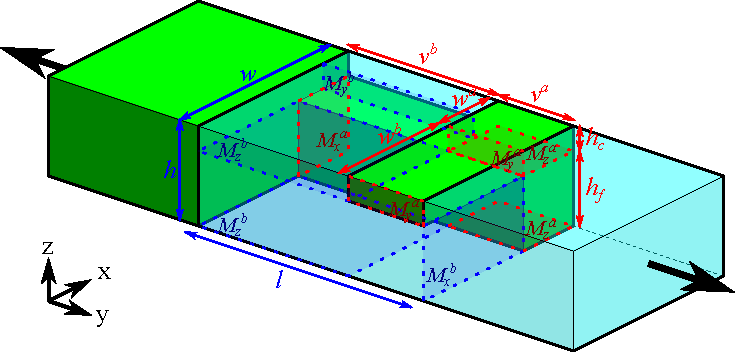
\includegraphics[width=\columnwidth]{sources/method/straight_model_v3.pdf}
	\caption{
		One straight unit cell connecting material $a$ (left) to material $b$ (right).
		Failure can happen along the fingers ($M_x$), along the cross beams ($M_y$) or at the interface between the two ($M_z$) for either material.}
	\label{fig:failure_modes}
\end{figure}

\begin{figure}[H]
	\centering
	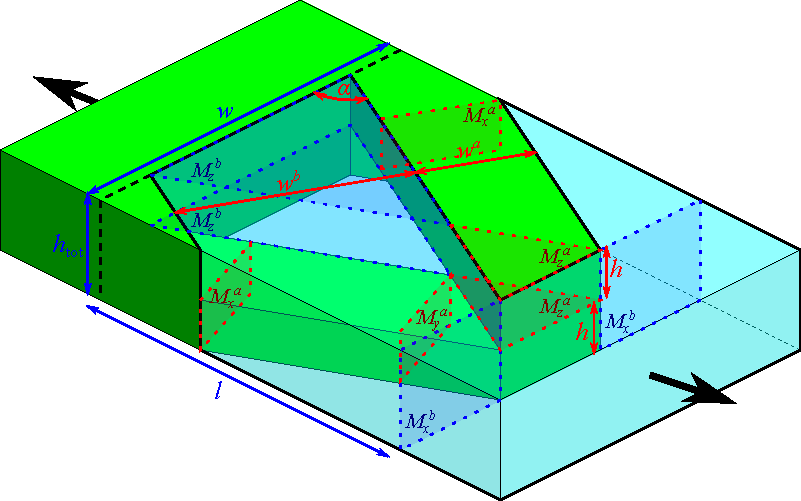
\includegraphics[width=\columnwidth]{sources/method/diagonal_model_v3.pdf}
	\caption{
		One diagonal unit cell connecting material $a$ (left) to material $b$ (right).
		Failure can happen along both the fingers ($M_x$), twice along one finger ($M_y$) or at the interface between the two fingers ($M_z$) for either material.}
	\label{fig:diagonal_model}
\end{figure}



\section{Straight Orientation}





\Cref{fig:failure_modes} shows one cell of the straight structure, along with the design variables and the failure modes.
The optimization then consists of the following:

\begin{align}
	& \max \frac{F}{\left( w^a + w^b \right) \left( h_\text{f} + h_\text{c} \right) } \\
	& \min h_\text{f} h_\text{c} \\
	\text{subject to} & \nonumber \\
	w^m &\ge w_\text{min}^m \\
	v^m &\ge v_\text{min}^m \\
	h_\text{f} &\ge h_\text{min} \\
	h_\text{c} &\ge h_\text{min} \\
	v^a + v^b &\le v_\text{max} \\
	\frac{ F }{ w^m h_\text{f} } &\le \sigma^m_\text{yield} &&\text{ Tension failure } M_x^m \\
	\frac{ 3 F }{ 4 v^m h_\text{c}} &\le \tau^m 			&&\text{ Shear failure } M_y^m \\
	\frac{ 3 F }{ 4 v^m w^m } &\le \tau^m_\text{Z} 			&&\text{ Shear failure } M_z^m \\
	\frac{ 3 F w^b }{ 4 \left( v^a \right)^2 h_\text{c} } &\le \sigma^a_\text{yield}			&&\text{ Bending failure } M_y^a \\
	\frac{ 3 F w^a }{ 4 \left( v^b \right)^2 h_\text{c} } &\le \sigma^b_\text{yield}			&&\text{ Bending failure } M_y^b \\
	& \text{for both materials } && m \in \{a, b\} \nonumber
\end{align}

\iffalse

\paragraph{Monotonicity Analysis}
\begin{align*}
	\min & 1 - \frac{F}{\left( w^a + w^b \right) \left( h_\text{f} + h_\text{c} \right) }
																		&& F^-, w^{a+}, w^{b+},  h_\text{f}^+, h_\text{c}^+\\
	\text{subject to} & \nonumber \\
	1 - \frac{w^m }{w_\text{min}^m} &\le 0    							&& w^{m-} \\
	1 - \frac{v^m }{w_\text{min}^m} &\le 0    							&& v^{m-} \\
	1 - \frac{h_\text{f}}{h_\text{min}} &\le 0 							&& h_\text{f}^- \\
	1 - \frac{h_\text{c}}{h_\text{min}} &\le 0 							&& h_\text{c}^- \\
	\frac{v^a + v^b}{ v_\text{max} }  - 1&\le 0 						&& v^{a+}, v^{b+} \\
	\frac{ F }{ w^m h_\text{f} \sigma^m_\text{yield} } - 1&\le 0 		&& F^+, w^{m-}, h_\text{f}^- \\
	\frac{ 2 F }{ 3 v^m h_\text{c} \tau^m } - 1 &\le 0 					&& F^+, v^{m-}, h_\text{c}^- \\
	\frac{ 2 F }{ 3 v^m w^m \tau^m_\text{Z} } - 1 &\le 0 					&& F^+, v^{m-}, w^{m-} \\
	\nonumber \\
	F^m &= \sigma^m w^m h_\text{f} \\
	\dots \\
	& \text{for both materials } m \in \{a, b\}
\end{align*}
\fi


This looks like a multi-objective optimization problem, but without the second objective the problem is under-constrained.
Adding the second objective actually means there's one unique solution - rather counter-intuitively.

The $v^m$ variables don't figure in the objective, but they do appear in the constraints and therefore are also subject to the optimization.

We should be able to find analytical solution(s), depending on the size of $v_\text{max}$ w.r.t. the other constraints.

Possible extensions:
\begin{itemize}
	\item Consider multiple repetitions of the cell in the loading direction.
	\item Consider tensile load in Z direction.
	\item Consider FEM model.
\end{itemize}

\iffalse
Formula is given by this? :
% from https://skyciv.com/docs/tutorials/beam-tutorials/bending-moment-equations/
\begin{align*}
	\sigma_\text{bend} &= \frac{M r}{I} \\
	&= \frac{M \nicefrac12 v}{I} \\
	M_\text{max} &= \frac{v L}{12} \text{ for distributed force and fixed sides} 
\end{align*}
\fi













\section{Slanted design}

Another option is to place the fingers under an angle as shown in \autoref{fig:diagonal_model}.
There are four design variables: the finger width of both materials: $w^a$ and $w^b$, the finger rotation angle $\alpha$, and the layer thickness $h$.




The goal is to maximize the strength, while accounting for the failure modes in the constraints.
With that, the optimization problem can be formulated as follows:

\begin{align}
	& \max \frac{F \sin \alpha}{\left( w^a + w^b \right) 2h } \\
	\text{subject to:} & \nonumber \\
	w^m &\ge w_\text{min}^m \\
	h &\ge h_\text{min} \\
	\alpha_{min} &\le \alpha \le \alpha_{max}\\
	w^a + w^b &\le w_\text{max} \\
	\frac{ F \sin \alpha}{ w^m h } &\le \sigma^m_\text{yield} &&\text{ Tension failure } M_x^m \\
	\frac{ 3 F \cos \alpha }{ 4 w^m h_\text{c}} &\le \tau^m 			&&\text{ Shear failure } M_x^m \\
	\frac{ 3 F \sin \alpha \cos \alpha }{ \left(w^m \right)^2 } &\le \tau^m_\text{Z} 			&&\text{ Shear failure } M_z^m \\
	\frac{ 3 F w^b }{ 8 \sin \alpha \left(w^a \right)^2 h} & \le \sigma^a_\text{yield}			&&\text{ Bending failure } M_x^a \\
	\frac{ 3 F w^a }{ 8 \sin \alpha \left(w^b \right)^2 h} & \le \sigma^b_\text{yield}			&&\text{ Bending failure } M_x^b \\
	& \text{for both materials } && m \in \{a, b\} \nonumber
\end{align}



\begin{figure}[H]
	\centering
	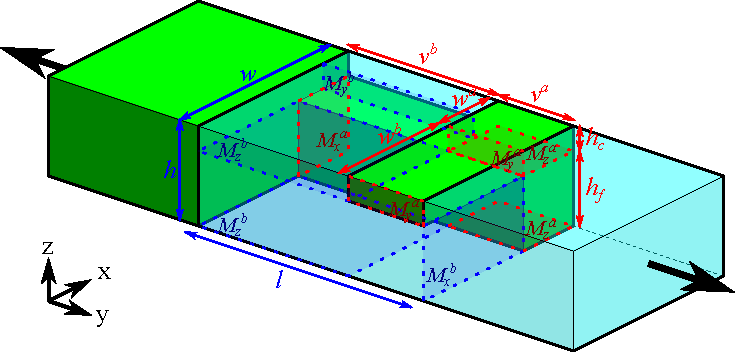
\includegraphics[width=\columnwidth]{sources/method/straight_model_v3.pdf}
	\caption{
		One straight unit cell connecting material $a$ (left) to material $b$ (right).
		Failure can happen along the fingers ($M_x$), along the cross beams ($M_y$) or at the interface between the two ($M_z$) for either material.}
	\label{fig:failure_modes}
\end{figure}


\section{Straight design}

\iffalse
The bending constraint is given by:
\begin{align*}
	\sigma_\text{max} &= \frac{M}{I}c \\
	c &= \nicefrac12 h \\
	I &= \frac{b h^3}{12} \\
	M &= \frac{w L^2}{8} \\
	w &= \frac{F}{L} \\
	\sigma_\text{max} &= \frac{12 F L}{8 b h^3} \nicefrac12 h \\
	\sigma_\text{max} &= \frac{3 F L}{4 b h^3} h \\
	\sigma_\text{max} &= \frac{3 F L}{4 b h^2} \\
\end{align*}
\fi


\Cref{fig:failure_modes} shows one cell of the straight structure, along with the design variables and the failure modes.
The optimization then consists of the following:

\begin{align}
	& \omit\rlap{$\displaystyle \max{ \frac{F}{\left( w^a + w^b \right) \left( h_\text{f} + h_\text{c} \right) }}$} \label{eq:obj} \\
% 	& \min{ h_\text{f} + h_\text{c}}
\omit\rlap{subject to} \nonumber \\
	w^m &\ge 2 w_\text{min}^m 								&&\text{ Nozzle size} \label{eq:c1} \\
	v^m &\ge w_\text{min}^m 								&&\text{ Nozzle size}  \label{eq:c2} \\
	h_\text{f} &\ge h_\text{min}  							&&\text{ Layer thickness}  \label{eq:c3} \\
	h_\text{c} &\ge h_\text{min} 							&&\text{ Layer thickness}  \label{eq:c4} \\
	v^a + v^b &\le l_\text{max} 							&&\text{ Design constraint}   \label{eq:c_total_length} \\
	\frac{ F }{ w^m h_\text{f} } &\le \sigma^m_\text{fail} &&\text{ Tension failure } M_x^m  \label{eq:c_tensile} \\
	\frac{ 3 F }{ 4 v^m h_\text{c}} &\le \nicefrac12 \sigma^m_\text{fail} 			&&\text{ Shear failure } M_y^m  \label{eq:c_shear} \\
	\frac{ 3 F }{ 4 v^m w^m } &\le \tau^m_\text{Z} 			&&\text{ Shear failure } M_z^m  \label{eq:c_shear_z} \\
	\frac{ 3 F w^b }{ 4 \left( v^a \right)^2 h_\text{c} } &\le \sigma^a_\text{fail}			&&\text{ Bending failure } M_y^a  \label{eq:c_bending_a} \\
	\frac{ 3 F w^a }{ 4 \left( v^b \right)^2 h_\text{c} } &\le \sigma^b_\text{fail}			&&\text{ Bending failure } M_y^b  \label{eq:c_bending_b} \\
	& \text{for both materials } && m \in \{a, b\} \nonumber
\end{align}

This looks like a multi-objective optimization problem, but without the second objective the problem is under-constrained.
Adding the second objective actually means there's one unique solution - rather counter-intuitively.

The $v^m$ variables don't figure in the objective, but they do appear in the constraints and therefore are also subject to the optimization.

Under different circumstances the values of the constraints will be different.
Because of manufacturing constraints we know that the layer thickness has to be smaller than half the smallest nozzle size:
$h_\text{min} < \nicefrac{1}{2} w^m_\text{min}$.
Depending on the design we might apply a different $l_\text{max}$, 
but it is required that $l_\text{max} \ge v_\text{min}^a + v_\text{min}^b$.
Materials properties of 3D printed materials are always such that $\tau_Z^m < \tau^m$.
Maximum shear stress theory further gives us that $\tau^m = \nicefrac12 \sigma^m_\text{fail}$.

Conversely, if $\nicefrac{w^b}{v^a} > \nicefrac{ \sigma^a_\text{fail} }{ \tau^a } = 2$ 
then the shear failure constraint \cref{eq:c_shear} is dominated by the bending failure constraint \cref{eq:c_bending_a},
since then 
$
\frac{ 3 F w^b }{ 4 \left( v^a \right)^2 h_\text{c} \sigma^a_\text{fail}}
> \frac{ 3 F }{ 4 v^a h_\text{c} \tau^a} 
$.
Otherwise the latter is dominated by the former.
The same holds conversely with the materials $a$ and $b$ swapped.
Therefore two of \cref{eq:c_shear}, \cref{eq:c_bending_a} and \cref{eq:c_bending_b} will be redundant.


Depending on the types of material used the tensile and shear strength in the Z direction can be an order of magnitude lower than in the horizontal directions.
In such a case the Z shearing failure constraint \cref{eq:c_shear_z} will be active for that material.



\subsection{Monotonicity Analysis}
\tim{TODO: Convert objective function into a minimization problem and flip the signs everywhere.}
\begin{align*}
	\max{ \frac{F}{\left( w^a + w^b \right) \left( h_\text{f} + h_\text{c} \right) } }
																		&& F^+, w^{a-}, w^{b-},  h_\text{f}^-, h_\text{c}^-\\
\omit\rlap{subject to} \nonumber \\
	1 - \nicefrac{w^m }{2 w_\text{min}^m} &\le 0    					& w^{m-} \\
	1 - \nicefrac{v^m }{w_\text{min}^m} &\le 0    						& v^{m-} \\
	1 - \nicefrac{h_\text{f}}{h_\text{min}} &\le 0 						& h_\text{f}^- \\
	1 - \nicefrac{h_\text{c}}{h_\text{min}} &\le 0 						& h_\text{c}^- \\
	\frac{v^a + v^b}{ l_\text{max} }  - 1&\le 0 						& v^{a+}, v^{b+} \\
	\frac{ F }{ w^m h_\text{f} \sigma^m_\text{fail} } - 1&\le 0 		& F^+, w^{m-}, h_\text{f}^- \\
	\frac{ 3 F }{ 4 v^m h_\text{c} \tau^m } - 1 &\le 0 					& F^+, v^{m-}, h_\text{c}^- \\
	\frac{ 3 F }{ 4 v^m w^m \tau^m_\text{Z} } - 1 &\le 0 				& F^+, v^{m-}, w^{m-} \\
	\frac{ 3 F w^b }{ 4 \left( v^a \right)^2 h_\text{c} \sigma^a_\text{fail} } - 1 &\le 0			& F^+, w^{b+}, v^{a-}, h_\text{c}^-\\
	\frac{ 3 F w^a }{ 4 \left( v^b \right)^2 h_\text{c} \sigma^b_\text{fail} } - 1 &\le 0			& F^+, w^{a+}, v^{b-}, h_\text{c}^-\\
	\text{for both materials } && m \in \{a, b\}
\end{align*}

If we would scale all design variables linearly with some factor $R$ and $F$ by $R^2$ then the objective function and all mechanical constraints \crefrange{eq:c_tensile}{eq:c_bending_b} remain at the same value.
If only those constraints were to be considered the problem would have been under-constrained.
Therefore some of the constraints \crefrange{eq:c1}{eq:c_total_length} will have to be active.
%incorrect! : Since only \cref{eq:c_total_length} provides an upper bound it must be active.
If we set \cref{eq:c1} active for material $a$ \todo{we will show} that none of the other constraints will be violated, so this constraint has to be active.



\subsection{Future work}
Possible extensions:
\begin{itemize}
	\item Consider how the optimal design depends on the constraint values.
	\item Test various material combinations.
	\item Consider multiple repetitions of the cell in the loading direction.
	\item Consider tensile load in Z direction.
	\item Consider FEM model.
\end{itemize}

\iffalse
Formula is given by this? :
% from https://skyciv.com/docs/tutorials/beam-tutorials/bending-moment-equations/
\begin{align*}
	\sigma_\text{bend} &= \frac{M r}{I} \\
	&= \frac{M \nicefrac12 v}{I} \\
	M_\text{max} &= \frac{v L}{12} \text{ for distributed force and fixed sides} 
\end{align*}
\fi




\begin{figure}[H]
	\centering
	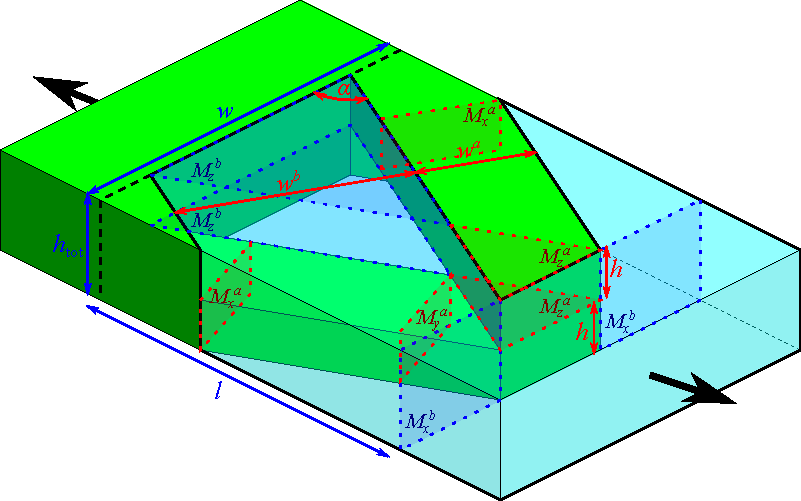
\includegraphics[width=\columnwidth]{sources/method/diagonal_model_v3.pdf}
	\caption{
		One diagonal unit cell connecting material $a$ (left) to material $b$ (right).
		Failure can happen along both the fingers ($M_x$), twice along one finger ($M_y$) or at the interface between the two fingers ($M_z$) for either material.}
	\label{fig:diagonal_model}
\end{figure}



\section{Diagonal Design}

Another option is to place the fingers under an angle as shown in \autoref{fig:diagonal_model}.
There are four variables: the finger width of both materials: $w_a$ and $w_b$, the length $L$ and the layer thickness $h$. If all four variables are scaled, then the objective function and the constrained functions scale with the same factor. Therefore, the layer thickness $h$ will be fixed to $h = h_{min}$ and only the variables $w_a$, $w_b$ and $L$ will be optimized.

\section{Problem Formulation}
This section shows the deriviation of the problem formulation.

\subsection{Geometry Relations}
From \autoref{fig:diagonal_model}, the geometry relations \ref{eq:tan}, \ref{eq:cos} and \ref{eq:sin} can be derived, which are used for further analysis of the stresses.

\begin{equation}
	\label{eq:tan}
	\tan \alpha = \frac{2L}{w_a + w_b}
\end{equation}

\begin{equation}
	\label{eq:cos}
	\cos \alpha = \frac{w_a + w_b}{\sqrt{ \left( w_a + w_b \right) ^2 + 4L ^2 }}
\end{equation}

\begin{equation}
	\label{eq:sin}
	\sin \alpha = \frac{2L}{\sqrt{ \left( w_a + w_b \right) ^2 + 4L ^2 }}
\end{equation}


\subsection{Tension Failure M$_x$}\label{ssec:tensfail}
For the tension failure, we consider the smallest cross sectional area of one finger, which is equal to $w_m h \sin \alpha$ . The tensile force perpendicular to this area is equal to $\frac{F}{\sin \alpha}$, where $F$ is the force per finger. %which was divided by 2 because every finger takes up half of the load. ? - adjust later maybe
Working out $\frac{F}{A} \le \sigma$ resulted in \autoref{eq:tensfail}


\begin{equation}
		\label{eq:tensfail}
	\frac{F}{w_m  h} \le \sigma_{max}
\end{equation}


\subsection{Shear Failure M\textsubscript{x}}
The same cross sectional area was taken as in \autoref{ssec:tensfail}, but now the force that is aligned with this cross section $F \cos \alpha$ is used to evaluate the shear forces. The maximum shear stress for a rectangular cross sectional area is equal to $\frac{3V}{2A}$. In this way, we derived \autoref{eq:shearfailtemp}

\begin{equation}
	\label{eq:shearfailtemp}
	\frac{3F \cos \alpha}{w_m h \sin \alpha} = \frac{3F }{w_m h \tan \alpha} \le \tau_m
\end{equation}

We plugged in \autoref{eq:tan} what resulted in \autoref{eq:shearmx}.
\begin{equation}
	\label{eq:shearmx}
	\frac{ 3 F \left(w_a + w_b \right) }{ 4  w_m h L} \le \tau_m	
\end{equation}

\subsection{Shear Failure M\textsubscript{z}}
For a triangular cross section, the maximum shear stress is equal to $\frac{3F}{bh}$, where $b$ and $h$ are the base and the height of the triangle. The width and height of the rectangular area that is loaded in shear are equal to $w_m$ and $\frac{w_m \tan \alpha}{2} $ respectively. Combining with \ref{eq:tan} gave \autoref{eq:shearMz}.

\begin{equation}
	\label{eq:shearMz}
	\frac{ 3 F \left(w_a + w_b \right) }{ w_m ^2 L} \le \tau_m	
\end{equation}


\subsection{Bending Failure M\textsubscript{x}}
The length of each finger, which we call $l$, is defined in \autoref{eq:l}

\begin{equation}
	\label{eq:l}
	l = \sqrt{ \frac{\left( w_a + w_b \right)}{2} ^2 + L^2 }
\end{equation}
Then we can derive the moment in \autoref{eq:momentder}.

\begin{equation}
	\label{eq:momentder}
	\frac{F \cos \alpha l}{2} =  \frac{F \frac{\left(w_a + w_b \right)}{2l} l}{2} = \frac{F \left(w_a + w_b\right)}{4}ent...
\end{equation}
The moment of inertia $I$ for the rectangular cross section is $\frac{h \left(w_m \sin \alpha \right)^3}{12}$. With $y = \frac{w_m \sin \alpha }{2}$, this gives a bending stress $\frac{M y}{I}$ as shown in \autoref{eq:bendingtemp}

\begin{equation}
	\label{eq:bendingtemp}
	\frac{3 F\left(w_a + w_b \right)}{2 h \left( w_m \sin \alpha \right)^2 } \le \sigma_m
\end{equation}

Then we replaced $\sin \alpha$ with \ref{eq:sin}, where \autoref{eq:bending} was the final result.

\begin{equation}
	\label{eq:bending}
	\frac{ 3 F \left(w_a + w_b \right) \left(\left(w_a + w_b \right) ^2 + 4L^2 \right)  }{ 8h w_m^2 L^2 }  \le \sigma_m
\end{equation}

\subsection{Von Mises Stress Criterion}
The tensile $\sigma_t$, bending $\sigma_b$ and shear stresses $\tau_x$ acting at the section $M_x$ were combined into the Von Mises stress criterion. The Von Mises stress is defined in \autoref{eq:vm}.

\begin{equation}
	\label{eq:vm}
	\sqrt{\frac{\left( \sigma_t + \sigma_b \right)^2}{2} + 3\tau_x ^2}
\end{equation}

We plugged in \autoref{eq:tensfail}, \ref{eq:shearmx} and \ref{eq:bending}, what gave \ref{eq:vmcrit}.

\begin{equation}
	\label{eq:vmcrit}
	\sqrt{\frac{1}{2} \left( \frac{F}{w_m  h} + 	\frac{ 3 F \left(w_a + w_b \right) \left(\left(w_a + w_b \right) ^2 + 4L^2 \right)  }{ 8h w_m^2 L^2 }   \right)^2+ 3\left(	\frac{ 3 F \left(w_a + w_b \right) }{ 4  w_m h L }  \right) ^2}
\end{equation}
\todo{How to put it on the page??} 


\subsection{Optimization Problem}
The goal is to maximize the strength while accounting for the failure modes in the constraints.
With that, the optimization problem can be formulated as follows:

\begin{align*}
	f: & \max_{F, {w_a}, {w_b}. L} \frac{F}{2h \left(w_a + w_b\right)} \nonumber \\
	\text{subject to:} & \nonumber \\
	g_1: & w_m \ge w_\text{m,min} \\
	g_2: & w_a + w_b \le w_\text{max} \\
	g_3: & L_{min} \le L \le L_{max} \\
	g_4: & \frac{ 3 F \left(w_a + w_b \right) }{ w_m ^2 L} \le \tau_m						\text{ Shear failure } M_z^m \\
	g_5:& \sqrt{\frac{1}{2} \left( \frac{F}{w_m  h} + 	\frac{ 3 F \left(w_a + w_b \right) \left(\left(w_a + w_b \right) ^2 + 4L^2 \right)  }{ 8h w_m^2 L^2 }   \right)^2+ 3\left(	\frac{ 3 F \left(w_a + w_b \right) }{ 4  w_m h L}  \right) ^2}		\le 	\sigma_m	\text{ Von Mises criterion } M_x \\
	& \text{for both materials } && m \in \{a, b\} \nonumber 
\end{align*}


Normalizing and rewriting to the negative null-form gives the following optimization problem:

\begin{align*}
	f: & \min_{F, {w_a}, {w_b}. L}  \frac{2h \left(w_a + w_b\right)}{F} \nonumber \\
	\text{subject to:} & \nonumber \\
	g_{1a}:& 1 - \frac{w_a}{w_{a,min}}  \le 0 \\
	g_{1b}:& 1 - \frac{w_b}{w_{b,min}}  \le 0 \\
	g_2:& \frac{w_a + w_b}{w_{max}}  - 1 \le 0 \\
	g_{3.1}:& 1 - \frac{L}{L_{min}} \le 0 \\
	g_{3.2}:&\frac{L}{L_{max}} - 1  \le 0 \\
	g_{4a}: & \frac{ 3 F \left(w_a + w_b \right) }{ \tau_a w_a ^2 L} - 1 \le 0					\text{ Shear failure } M_z^a \\
	g_{4b}: & \frac{ 3 F \left(w_a + w_b \right) }{ \tau_b w_b ^2 L} - 1 \le 0					\text{ Shear failure } M_z^b \\
	g_{5a}:& \frac{\sqrt{\frac{1}{2} \left( \frac{F}{w_a  h} + 	\frac{ 3 F \left(w_a + w_b \right) \left(\left(w_a + w_b \right) ^2 + 4L^2 \right)  }{ 8h w_a^2 L^2 }   \right)^2+ 3\left(	\frac{ 3 F \left(w_a + w_b \right) }{ 4  w_a h L}  \right) ^2}	} { \sigma_a} - 1	\le 0	\text{ Von Mises criterion } M_x^a \\
	g_{5b}:& \frac{\sqrt{\frac{1}{2} \left( \frac{F}{w_b  h} + 	\frac{ 3 F \left(w_a + w_b \right) \left(\left(w_a + w_b \right) ^2 + 4L^2 \right)  }{ 8h w_b^2 L^2 }   \right)^2+ 3\left(	\frac{ 3 F \left(w_a + w_b \right) }{ 4  w_b h L}  \right) ^2}	} { \sigma_b} - 1	\le 0	\text{ Von Mises criterion } M_x^a 
\end{align*}
\todo{How to put it neatly on one line?}



\subsection{Modelling Aspects}
One of the modelling aspects that should be considered is that all fingers are modelled as a cantilever beam with a distributed load. It is assumed that every finger takes up the same load $F$, still one finger will fail earlier than the other because of a difference in the stress levels. Furthermore, the Von Mises stress criterion was used to predict the yielding of the material under multiple loading conditions. This does not account for the an-isotropic nature of the 3D printed material, neither for the lower infill density if larger regions are considered. It should also be noted that the adhesive bonds between the layers are weaker in shear $M_z$ compared to the nominal shear strength. Therefore, this study should only be used as an initial investigation which needs to be tested and tuned in any case.

\section{Initial Problem Investigation}
This section discusses the initial investigation of the optimization problem. 

\subsection{Boundedness}
The optimization problem aims to maximize the strength, which scales proportionally with $F$ and inversily with the total width $w_a + w_b$ and the layer height $h$.  $f$ is minimized if $w_a + w_b$ and $h$ are approaching zero and if $F$ goes to infinity. Since the minimizers $F*$, $w_a*$, $w_b*$ and $L*$ do not lie within the set of positive and finite numbers $P$, the objective function is not well bounded for any of the design variables and therefore constraints are needed. The layer height $h$ was fixed and a lower bound was set on $w_a$ and $w_b$ with manufacturing constraint $g_1$. In addition, the finger length $L$ was bounded between $L_{min}$ and $L_{max}$ in constraint $g_3$, and $g_4$ and $g_5$ put an upper bound on the force $F$ that the fingers can withstand. 

\subsection{Convexity}
The objective function $f$ and the constraints $g_1$, $g_2$ and $g_3$ are linear and therefore also convex. For constraint $g_4$, the Hessian matrix was evaluated, where all principle minors should be positive semi-definite for the function to be convex. A 3x3 principle minor of the full 4x4 Hessian of $g_{4a}$ is given in \autoref{eq:Hg4} with partial derivatives for the design variables $L$, $w_a$ and $w_b$.

\begin{equation}
	\label{eq:Hg4}
	H = \begin{bmatrix}
				 g_{wa, wa} & g_{wa, wb} & g_{wa, L} \\
				 g_{wb, wa} & g_{wb, wb} & g_{wb, L}  \\
				 g_{L, wa} & g_{L, wb} & g_{L, L} 													
		\end{bmatrix}
	= \frac{3F}{\tau_a}\begin{bmatrix}
		\frac{2w_a + 6 w_b}{\left( w_a \right)^4 L} & \frac{-2}{\left( w_a \right)^3 L } &  \frac{w_a + 2 w_b}{\left( w_a \right)^3 L^2 }\\
		\frac{-2}{\left( w_a \right)^3 L } & 0 & \frac{1}{\left( w_a \right)^2 L^2 }  \\
\frac{w_a + 2 w_b}{\left( w_a \right)^3 L^2 } & \frac{1}{\left( w_a \right)^2 L^2 } & \frac{2 \left(w_a + w_b\right)}{\left( w_a \right)^2 L^3}													
	\end{bmatrix}
\end{equation}

The principle minor of the upper-right 2x2 matrix of the Hessian: $\frac{-2}{\left( w_a \right)^3 L } \frac{1}{\left( w_a \right)^2 L^2 } - 0 $ is not negative, which implies non-convexity of constraint $g_4$.\\

Inside the square root of constraint $g_5$, there is a bending equation contains the same dependency as $g_4$ and then multiplied with even more terms. This clearly implies a non-convex constraint as well. \\
Besides the convex objective function, the feasible domain can have multiple local boundary optima because of the non-convex constraints $g_4$ and $g_5$. This should be accounted for during the optimization of the problem.

\subsection{Monotonicity}
A monotonicity analysis was performed, the results are displayed below. 
\begin{align*}
	f: & F^-, w_a^+, w_b^+ \\
	g_{1a}:& w_a^- \\
	g_{1b}:& w_b^- \\
	g_{2}:& w_a^+, w_b^+\\
	g_{3.1}:& L^- \\
	g_{3.2}:& L^+ \\
	g_{4a}:& F^+, w_a^-, w_b^+, L^- \\
	g_{4b}:& F^+, w_a^+, w_b^-, L^-\\
	g_{5a}:& F^+, w_b^+, L^-\\
	g_{5b}:& F^+, w_a^+, L^-
\end{align*}

The objective function is monotonically decreasing for $F$, and $F$ is monotonically increasing in constraint $g_{4a}$, $g_{4b}$, $g_{5a}$ and $g_{5b}$. This implies that one of these should be active. Similarly, $w_a$ and $w_b$ are monotonically increasing in the objective function. Therefore, constraints $g_{1a}$, $g_{1b}$, $g_{4a}$ or $g_{4b}$ should be active for $w_a$ or $w_b$. $L$ does not appear in the objective function but shall still be bounded within $L_{min}$ and $L_{max}$, to minimize the bending moment it is to be expected that $L$ is close to its minimum value. 

\subsection{Numerical Noise}
tbc.


\subsection{Sensitivity Analysis}
The logarithmic sensitivities were evaluated to compare the relative importance of each design variable on the objective function and the constraints. Since all variables in the constraints and in the objective function are independent from each other, there are no response variables that should be accounted for. \\
The sensitivities from constraints $g_1$ untill $g_4$ were obtained by evaluating the partial derivatives. 

\begin{align*}
\diff{_L f}{_L w_a} &= \frac{w_a}{w_a + w_b} \\
\diff{_L f}{_L w_a} &= \frac{w_b}{w_a + w_b} \\
\diff{_L f}{_L F} &= -1 \\
\diff{_L g_1}{_L w_a} &= t.b.c. \\
\end{align*}


\section{Initial Optimization}
For the initial optimization, the grid search method was used first, after which random jumping was performed within a smaller range around the optimum found by the former mentioned method. We choose this search method because the optimum found can be used as the starting point in the optmization of the actual problem. In addition, it is easy to implement, does not suffer from getting stuck into optima and does not require the functions to be linearlized with a Taylor series approximation. It can directly be implemented to optimize the four design variables $F$, $w_a$, $w_b$ and $L$. A disadvantage is that random search does not give an accurate solution if not many points are sampled, therefore the actual optimization will be done with another method. \\

We did the grid search for $w_a$ and $w_b$ ranging from 0.3 to 0.9mm with a step size of 0.1, $L$ from 1.8 to 4.6mm with a step size of 0.3, and $F$ from 1 N to 10 N with a step size of 0.25. The this resulted in a minimum objective value of 0.52 mm$^2$/N, obtained for the variables as indicated below.

\begin{align}
	w_a* &= 0.4\\
	w_b* &= 0.9 \\
	L* &= 3.6 \\
	F* &= 2.5 
\end{align} 


\section{Optimization of the Actual Problem}


\section{Optimization Approach}
Because of the specifics of our problems definitions we have chosen Sequential Quadratic Programming (SQP) as the optimization approach.
Given that our problems are constrained, none of the unconstrained optimization methods applies.
Also, given that the objective function and all of the stress values are monotonic, we expect the response surface not to be highly irregular, so random methods would be overkill.
In fact, we expect there to be one global optimum.
SQP seems a good candidate for an optimization approach because our objective function and constraints are differentiable and because it can deal with infeabile points natively.



\subsection{Implementation}

\newcommand{\xvec}{\mathbf{x}}
\newcommand{\hvec}{\mathbf{h}}
\newcommand{\gvec}{\mathbf{g}}
\newcommand{\Wmat}{\mathbf{W}}
\newcommand{\Amat}{\mathbf{A}}
\newcommand{\lamvec}{\bm{\lambda}}

Our objective and constraint formulae are differentiable,
but deriving the derivative of the more complex constraints may prove to be laborsome and error-prone.
We therefore use the Matlab builtin functionality \verb|diff| to derive the derivatives of the symbolic formulae.
Performing the differentiation like this is computation intensive, but since it can be performed at the start of the program we can save on precious computation time inside the main loop.
Inside the loop we evaluate the symbolic expressions of the derivatives using \verb|subs| and \verb|eval|.

The $\Wmat$ and $\Amat$ matrices can then be constructed on the fly using the formulae
$\Wmat = \diffp[2]{f}{\xvec} + \lamvec^\intercal \diffp[2]{\hvec}{\xvec}$
and
$\Amat = \diff{\hvec}{\xvec}$.
Note that $\diffp[2]{\hvec}{\xvec}$ is a precomputed 3D matrix.
We can then use \verb|quadprog| to solve $\min_{\Delta\xvec} \nicefrac12 \Delta\xvec^\intercal \Wmat\Delta\xvec + \nabla f^\intercal \Delta\xvec$ s.t. $\Amat\Delta\xvec+\hvec=\mathbf{0}$.

\subsubsection{Active set}
It was chosen to implement an active set strategy, because using slack variables or using penalty or barier functions introduces inaccuracies in the final result.
Here $\hvec$ is an active subset of all constraints $\gvec$, which is determined in each iteration based on the current $\xvec_k$.
One simple approach would be to set all constraints active which are violated by the current $\xvec_k$.
In order to be lenient to numerical errors we set a constraint $g_i$ as active when $g_i > -10^{-4}$.
This way successive iterations along a constraint boundary won't oscillate the active set.

However, such an approach can lead to problems when considering points near or beyond the global optimum.
When the active set contains more constraints than design variables, the quadratic program is unsolvable.
In an N-dimensional space only N hypersurfaces generally intersect in a point.
We feel that SQP is not inherently equipped to deal with an active set larger than the design space.

One naive approach to alleviate the issue is to choose the subset of the most violated constraints.
However, this will not work, since the optimization will only push $\xvec_k$ further from the ignored constraints if that is in favor of the objective function.
We did not develop any strategy to deal with this problem;
the program terminates prematurely with an error message in such a case.

\subsubsection{Lagrange multipliers}
In order to compute the lambda multipliers of the outer problem we solve the system of linear equations given by
$\Amat_k =  - \Wmat_k  \Delta\xvec - \left[\nabla f\right]_k
$

Because the active set can change each iteration, the lambda values of constraints which were unused in the previous iteration might have to be revived.
We keep track of a set of Lagrange multipliers out of which the active subset is used each iteration.
We store the lambda values of the previous iteration in the full set, update the active set and then retrieve the new set of multipliers.

However, because the lambda values signify the relative importance of the constraints w.r.t. each other, the lambda values of one set cannot be reliably compared to another active set from the previous iteration.
We therefore set $\lamvec = \mathbf{1}$ whenever the active set changes.

\subsubsection{Instability prevention}
In some cases the optimization can oscillate between two constraints.
It can happen that the optimizatoin cycles between points on either side of two constraint surfaces.
Each time the optimization is in a point $\xvec_k$ which violates some constraing $g_a$,
it doesn't violate the other constraint $g_b$, which is then ignored;
the next iteration is then the other way around and thus a cycle is created.
However, this type of cycle is a cycle in the active set, not in $\xvec$.
We therefore invented a strategy to see if there is a cycle of 2 in the active sets of the past 6 iterations.
If there is, we force the active set to be the union of the 2 active sets in the cycle.
The forced active set is alleviated after 6 iterations, so that new constraints can come into view of the optimization.

Another problem which often occurs in one of the first iterations is that the update $\Delta\xvec$ becomes too large.
The optimization can then quickly escalate.
We therefore implemented a simple type of move limits: the magnitude of $\Delta\xvec$ was constrained to a maximum Euclidean length of 1.




\subsubsection{Stopping criteria}
The main loop of the optimization method is concluded when either of several criteria is met.
We break the loop when the improvement in one iteration is too small: $\left| \Delta\xvec \right| < \bm{1} \cdot 10^{-10}$.
In order to stop even earlier than that we also check the KKT conditions every iteration.
We can use \verb|linsolve| to get a full set of Lagrange multipliers to satisfy the optimality criterion
and verify whether the feasibility and complementarity constraints are satisfied.
However, using the approximate $\lamvec$ seems to give the same results.


In other cases the main loop is terminated because the optimization failed.
In order to prevent an infinite loop, we set the maximum number of iterations to 500.
Also, in case there are more active constraints than design variables,
the \verb|quadprog| algorithm would fail with an error about Non-convexity,
because of problems with the active set as noted above.
We also implemented a typical cycle detection, based on the values of $f$ and $\xvec$.
If the difference between a point $\xvec_k$ and $\xvec_j$ is smaller than $10^{-4}$ in all dimensions of $\xvec$ and $f$ then execution is halted.
In order to prevent the failure, our program terminates prematurely with an error message.


\section{Initial Optimization}
This section describes the initial optimization on the simplified problem with two variables. All other variables were set to constant values in the feasible domain. 
\subsection{Straight Design}
Two variables: $w_b$ and $F$ were optimized to investigate the implementation of the SQP algorithm. The other variables, $h_f$, $v_a$ and $v_b$ were set to 1.0, 2.0 and 1.0 respectively such that these lie inside the feasible domain. The starting point was set to $[w_b F] = [1, 1]$ and the SQP algorithm was executed. The result is shown in \autoref{fig:straightopt}. As can be seen, the algorithm converges along constraint $g_{ca}$ towards the optimum of $[w_b F] = [2.25 23.56]$ mm, N. The minimized value of the objective function is then 0.145 mm$^2$/N, thus the maximum strength equals 6.90 N/mm$^2$ for this configuration. Constraints $g_{ca}$ and $g_{tb}$ are active. It takes 152 iterations till convergence. The SQP algorithm iterates in the infeasible domain as well, however this was as expected.


\begin{figure}[H]
	\centering
	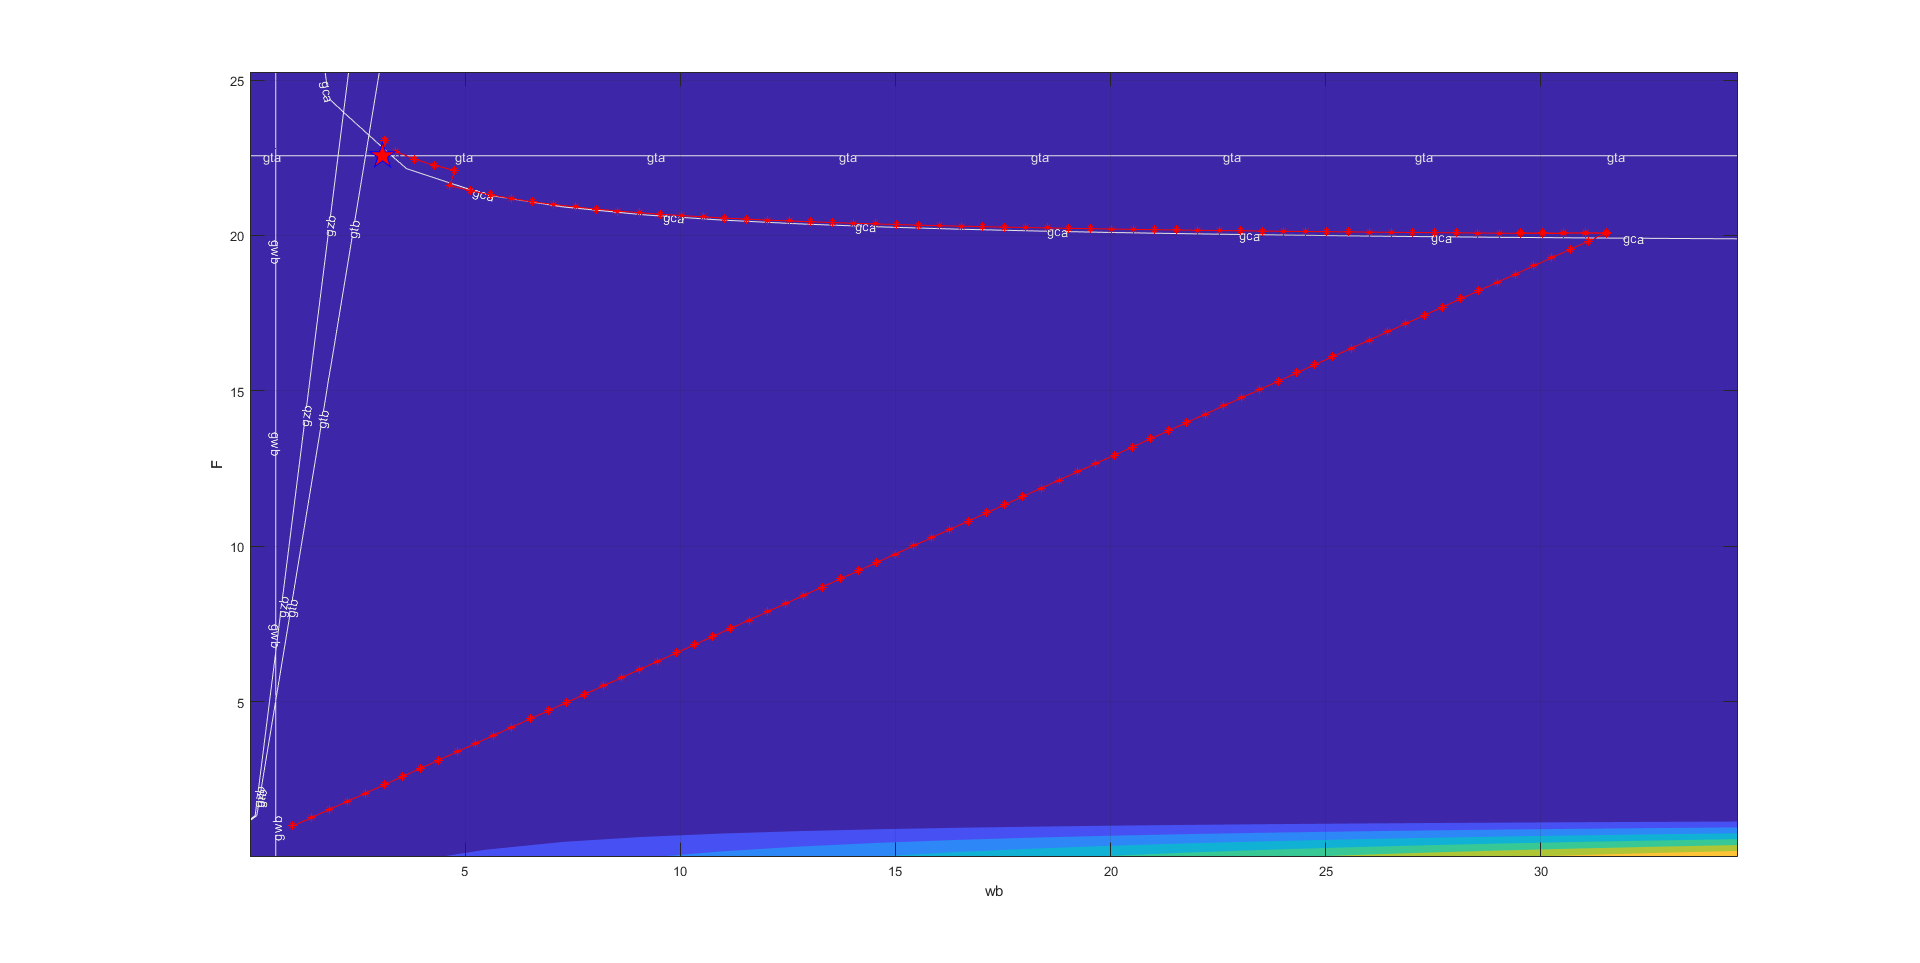
\includegraphics[width=\columnwidth]{sources/plots/straight2var.png}
	\caption{The optimization steps taken by the SQP algorithm for the design variables $w_b$ and $F$ in the straight design. The dashed line shows the infeasible domain.}
	\label{fig:straightopt}
\end{figure}


The KKT conditions were also checked. The feasibility conditions are satisfied because all inequality constraints are smaller than zero. Constraints $g_{ca}$ and $g_{tb}$ are treated as active, setting $\frac{\partial L}{\partial x} = 0$ gives two Lagrangian multipliers $\mu$ of 0.03 and 0.116. Since $\mu$ > 0, the KKT conditions are satisfied. Still, since not all constraint functions are convex, we cannot conclude that this is the global optimum from the KKT conditions merely. However, when looking at contour plot, the found optimum seems to be the global optimum since it lies just in the feasible domain and minimizes the objective function. 


\subsection{Diagonal Design}
The same SQP algorithm was also tested on the diagonal design. Again, $w_b$ and $F$ were optimized with an initial value of $[w_b F] = [1, 1]$. The other design variables $w_a$ and $L$ were set to 1.0 and 3.0 respectively. \autoref{fig:diagopt} shows the result, where $w_b$ and $F$ converge to 2.36 mm and 4.59 N respectively. This gives a minimized objective of 0.732 mm$^2$/N, equal to a maximum strength of 1.37 N/mm$^2$. Constraint $g_{5a}$ and $g_{5b}$ are then active and it takes 21 iterations till the optimum is found.


\begin{figure}[H]
	\centering
	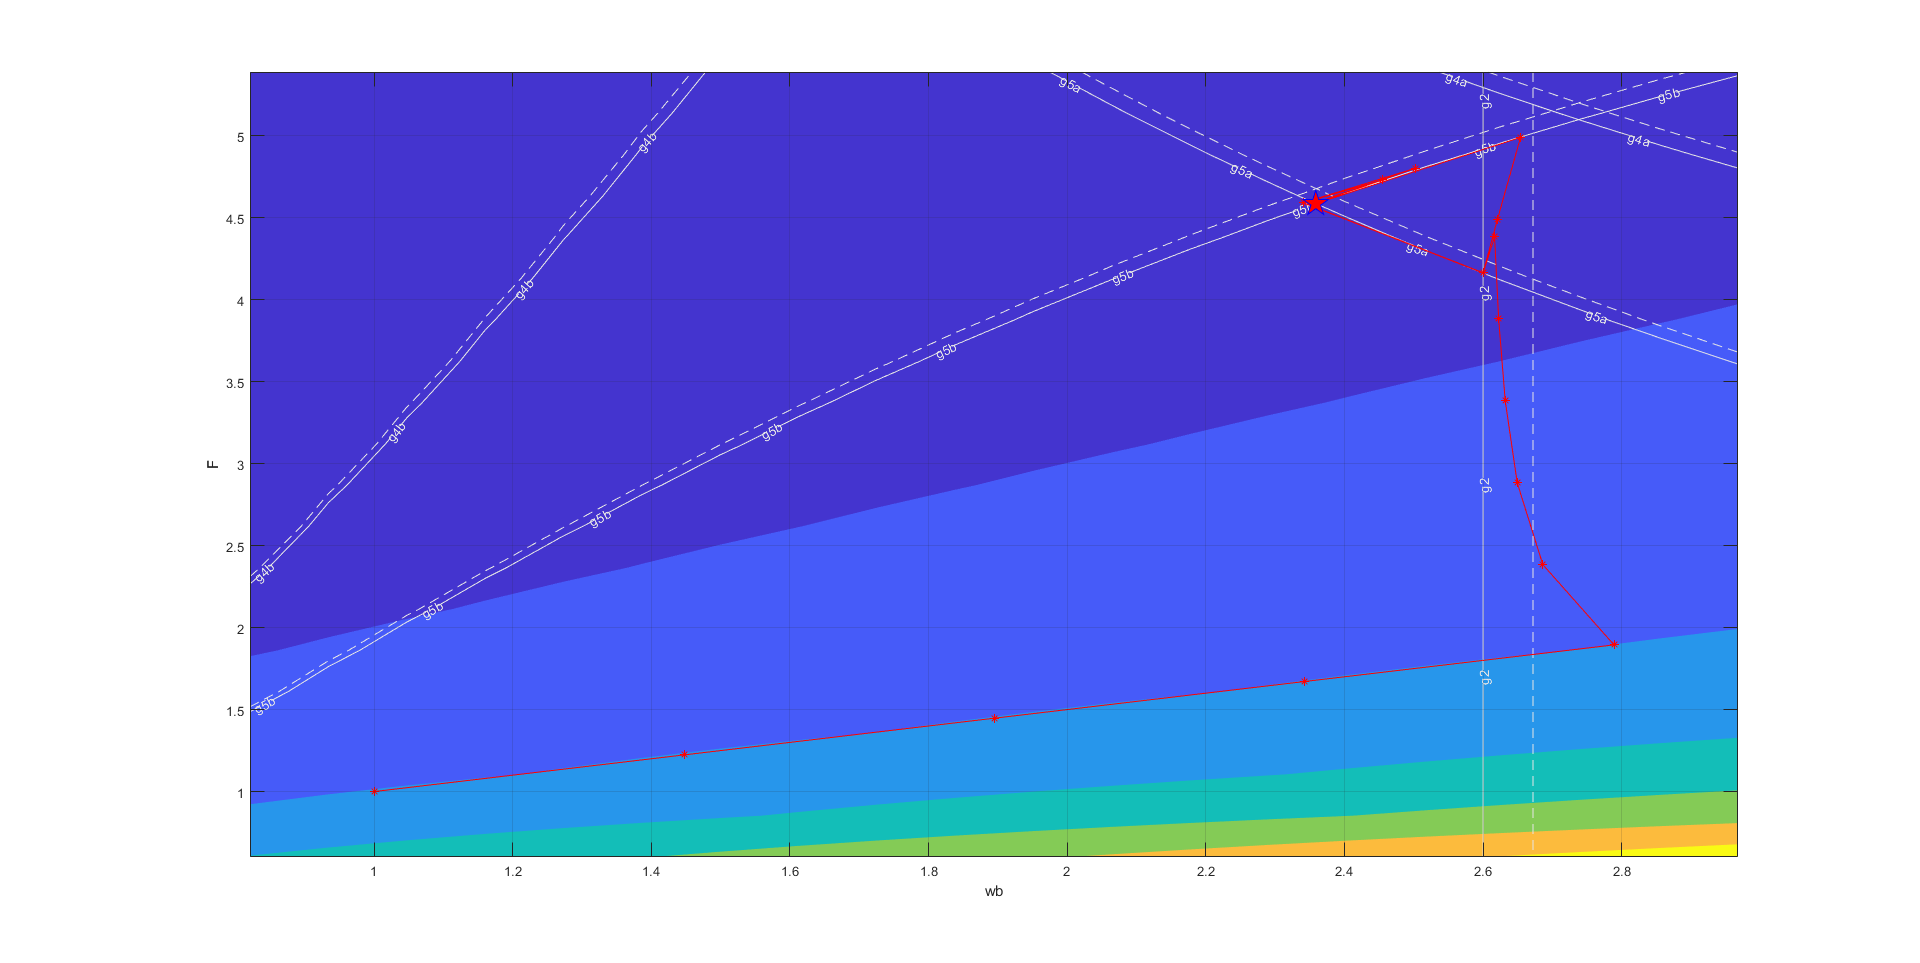
\includegraphics[width=\columnwidth]{sources/plots/diagonal2var.png}
	\caption{The optimization steps taken by the SQP algorithm for the design variables $w_b$ and $F$ in the diagonal design. The dashed line shows the infeasible domain.}
	\label{fig:diagopt}
\end{figure}

Looking at the KKT conditions, the optimum lies in the feasible domain since all inequality constraints are smaller than zero, and therefore satisfied. Treating constraints $g_{5a}$ and $g_{5b}$ as active gives two Lagrangian multipliers $\mu$ of 0.15 and 0.73. Since $\mu$ > 0, the KKT conditions are satisfied and the SQP algorithm has found a local optimum. Still, the constraints are not convex so it cannot be concluded that this is a global optimum from the KKT conditions only. Observing the contour plot, it can be seen that the objective function is minimized at the optimum found, and all constraints are satisfied. Therefore, the SQP algorithm found a global optimum in this case as well.\\

Note that the maximum strength values for the straight vs diagonal design are not comparable yet, since the other design variables were set at an arbitrary value in the feasible domain.










\section{Actual Optimization}
\subsection{Straight Case}
The full optimization problem was run with the same SQP implementation. After 184 iterations, the algorithm converged to an optimum of 0.137971 mm$^2$/N, equal to a maximum strength of 7.247898 N/mm$^2$. The values for the variables are presented in \autoref{tab:straightres}. It can be observed that the own implemenation of the SQP algorithm converges towards the same optimum, the deviation is in the order $10^{-3}$. The reason that the results do not exactly match is because of the discrete steps $dx$ taken by the SQP algorithm, the step size is in the order of $10^{-3}$ in the last iteration. 


\begin{table}[H]
	\centering
	\resizebox{\textwidth}{!}{%
		\begin{tabular}{|c|c|c|}
			\hline
			\textbf{Variable}           & \textbf{SQP - Own implementation}                                                       & \textbf{SQP - fmincon}                                                                  \\ \hline
			\textbf{Objective}          & 0.137971                                                                                & 0.137964                                                                                \\ \hline
			\textbf{Active constraints} & \begin{tabular}[c]{@{}c@{}}$g_d$, $g_{ta}$, $g_{tb}$,\\ $g_{ca}$, $g_{zb}$\end{tabular} & \begin{tabular}[c]{@{}c@{}}$g_d$, $g_{ta}$, $g_{tb}$,\\ $g_{ca}$, $g_{zb}$\end{tabular} \\ \hline
			\textbf{$w_b$}              & 2.683021                                                                                & 2.685714                                                                                \\ \hline
			\textbf{$v_a$}              & 2.667245                                                                                & 2.668029                                                                                \\ \hline
			\textbf{$v_b$}              & 0.932755                                                                                & 0.931971                                                                                \\ \hline
			\textbf{$h_f$}              & 1.087310                                                                                & 1.086396                                                                                \\ \hline
			$F$                         & 30.631543                                                                               & 30.636365                                                                               \\ \hline
		\end{tabular}%
	}
	\caption{The result of the own implementation of the SQP algorithm vs the MATLAB SQP solver fmincon.}
	\label{tab:straightres}
\end{table}


Then the KKT conditions were checked. The optimum lies in the feasible domain since all constraints are equal to or smaller than zero. Constraints $g_d$, $g_{ta}$, $g_{tb}$,\\ $g_{ca}$ and $g_{zb}$ are active.  It is remarkable that only three instead of five multipliers had a non-zero value, namely 0.0252, -0.00394 and 0.138. This can be caused by the order of accuracy of the implementation. While the constraints are considered to be active when they lie near zero, the actual value of the constraints lies in between +-$10^{-4}$ and +- $10^{-11}$. The 


\subsection{Diagonal Case}
-Nadine

\subsection{Discussion and Recommendations}
\subsection{Interpretation}
- Nadine
- Comparison fmincon
- KKT conditions checking
- Sensitivities (importance of constraints, variables)


\subsection{Recommendations}
Based on the maximum stress values of both optimizations is safe to assume that the straight interlocking design can outperform the diagonal design.
The maximum stress which can be reached with the straight design is roughly tripple the maximum stress which can be achieved using the diagonal setup.
Even when taking into account inaccuracies in the modeling (as discussed below) the straight design comes out as a clear winner.

The ultimate tensile strength of the interlocking metamaterial microstructure is predicted to be \SI{70}{\percent}
compared to the weaker of the two materials, Ultimaker PolyPropylene.
This value is relatively high compared to the weak chemical bonding between PP and most other thermoplastics.

Given that any manufacturing system has inaccuracies, it might be a good idea to settle on a design which is slightly different from the obtained optimum.
We can assume a deposition accuracy of \SI{0.1}{\milli\meter}, which is a reasonable guesstimate for most desktop FDM 3D printing systems.
The optimum is found at the intersection of several constraint surfaces - each of which has a different steepness at the optimum.
Taking the manufacturing accuracy is a random perturbation in the design space we can envision that the expected stress at the optimum might be lower
compared to a different reference point which is a bit farther down along the least steep surface.
Looking at the graphs and the sensitivities it would make sense to choose a design with a slightly lower $\hf$ and $w^b$ than the optimum of the straight design.
However, a thorough mathematical justification of the exact location of the best point in the design space given manufacturing inaccuracy remains future work.

Depending on the application of the interlocking structure different constraint values might apply.
For different materials the optimum can be quite different.
\todo{Refer to sensitivity wrt $\sigma_a$}
Another important consideration is the design constraint;
for thin designs the value of \SI{3.6}{\milli\meter} might be too big already.
\cref{fig:stress_vs_L} shows that if the design it, using a more lenient design constraint provides dimishing returns.
Moreover, the minimal manufacturable design is already at \SI{84}{\percent} of the ultimate stress compared to twice the total allowed length $\lmax$.

\begin{figure}
	\centering
	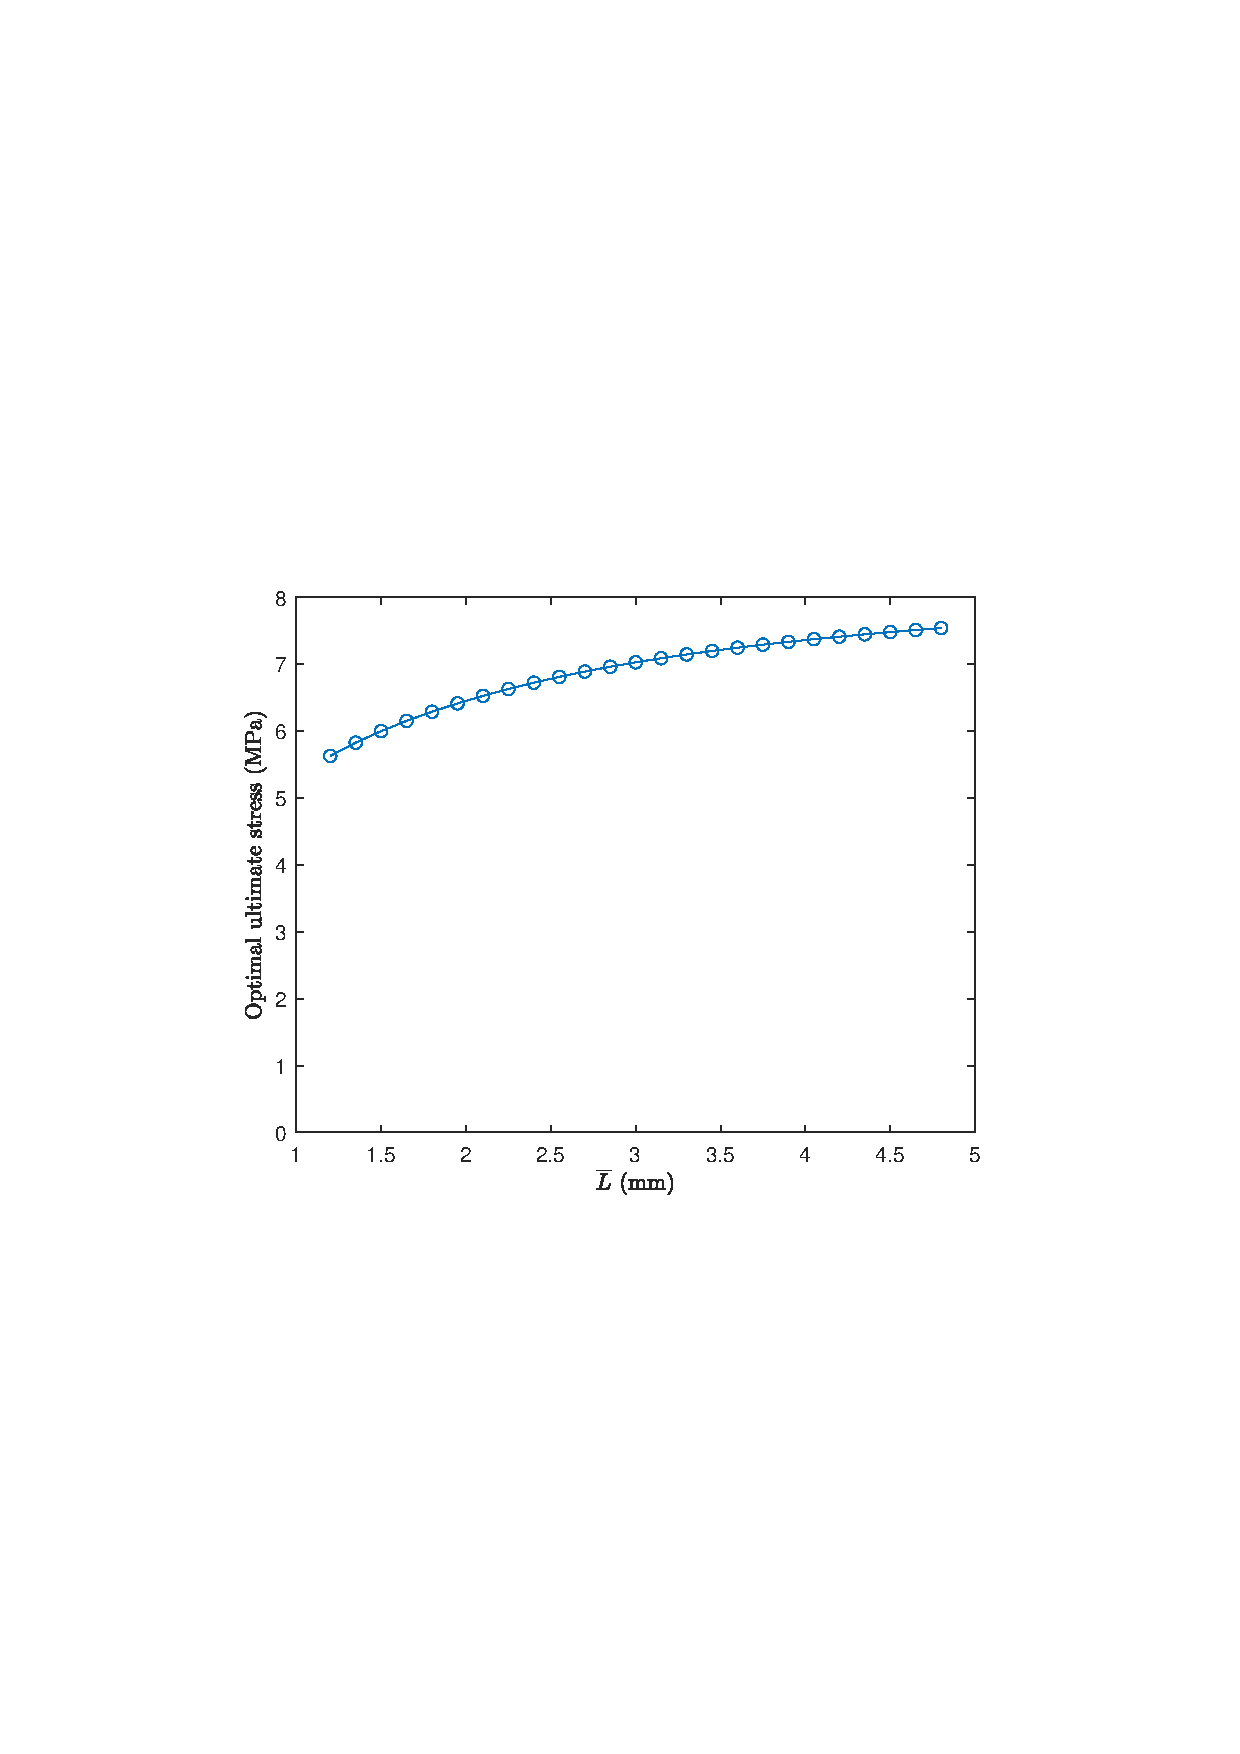
\includegraphics[width=.5\columnwidth]{sources/method/straight_max_stress_different_L.pdf}
	\caption{Optimal stress for various values of the design constraint.}
	\label{fig:stress_vs_L}
\end{figure}


\subsection{Limitations and Future work}
As mentioned before, the active set strategy and the lambda update strategy need more tuning to work properly;
if not with better heuristics then with local iterations to get $\xvec$ and $\lamvec$ closer to their intended values.

The mathematical problem definition we proposed has strong assumptions w.r.t. the homogeneity of stress distributions throughout the part,
while we can expect that in such complex internal loading scenarios the disctribution of stress to be heterogenous.
Specifically the validity of the diagonal model is hard to verify, given that the angles make for a difficult to analyse design.
Also factors such as friction can prove to be significant.

One line of future research is directed at different types of interlocking designs.
Does high genus interlocking designs outperform 2D dovetail type interlocking designs for more flexible materials?
How would the optimal interlocking design look for different forces, like shear, or a vertically applied force?

\subsection{Conclusion}
Tim




%\section*{References}
\interlinepenalty=100000 % prevents pdfendlink ended up accross pages error. see https://tex.stackexchange.com/a/449633/129190
\bibliography{99_mybib}


%\begin{appendices}
%\input{19_edge_discretization}
%\end{appendices}

\end{document}
